\section{Auswertung}
\label{sec:Auswertung}

Zunächst wird der Acrylblock mit einer Schieblehre vermessen.
Die Messwerte für die einzelnen Löcher sind in Tabelle \ref{tab:schieblehre} dargestellt.
Die Nummern der Bohrungen können der Abbildung \ref{fig:kenblock} entnommen werden.
Die Abmessungen des Blockes lauten:

\begin{align*}
  \text{Breite} &= \SI{150.25}{\milli\metre} \\
  \text{Höhe}   &= \SI{80.45}{\milli\metre} \\
  \text{Tiefe}  &= \SI{40.00}{\milli\metre}
\end{align*}

Wichtig ist für die folgenden Veruchsteile lediglich die Höhe des Blockes.

\begin{table}
  \centering
  \caption{Abmessungen der Bohrungen innerhalb des Acrylblockes.}
  \label{tab:schieblehre}
  \begin{tabular}[t]{c c c c}
   \toprule
    {Nummer} & {$l_\text{oben}$ / $\si{\milli\metre}$} & {$l_\text{unten}$ / $\si{\milli\metre}$} &  {Dicke / $\si{\milli\metre}$} \\
     \midrule
     \csvreader[no head,
     late after line=\\,
     late after last line=\\\bottomrule]%
     {data/abmessungentab.csv}{}%
     {$\num{\csvcoli}$ & $\num{\csvcolii}$ & $\num{\csvcoliii}$ & $\num{\csvcoliv}$ }%
   \end{tabular}
 \end{table}

\FloatBarrier
\subsection{Untersuchung eines Acrylblockes mit dem A-Scan}

Die Laufzeit der Schallwellen durch den Acrylblock bis zu der Störstelle ist in Tabelle \ref{tab:ascan} dargestellt.
Für die Umrechnung der Zeiten in die Länge wird Gleichung \eqref{eqn:wegzeit} genutzt.
Die Schallgeschwindigkeit in Acryl beträgt dabei $\SI{2730}{\metre\per\second}$ \cite{acryl}.
Da die Sonde nicht unmittelbar auf dem Acrylblock ruht, sondern auf einem Film aus bidestilliertem Wasser muss aus jeder Rechnung die Zeit herausgerechnet werden, die der Ultraschall benötigt um das Koppelmittel zu durchqueren.
Dieser wurde zu $\SI{0.43}{\micro\second}$ bestimmt.
Für die Bestimmung der Dicke der Bohrungen wird erneut die Dicke des Acrylblockes benötigt.
Die Gesamtzeit, die der Ultraschall benötigt um den Block zu durchqueren beträgt $\SI{60.55}{\micro\second}$, bzw. $\SI{60.12}{\micro\second}$ unter Berücksichtigung des Kopplungsmittels.
Damit lässt sich die Höhe des Blockes auf $\SI{82.06}{\milli\metre}$ berechnen. Durch Vergleich mit der, mitels Schieblehre, gemessenen Höhe von $\SI{80.45}{\milli\metre}$ wird die Dicke der Schutzschicht der Sonde zu
$\SI{1.61}{\milli\metre}$ bestimmt. Diese wird nun von allen bestimmten Längen abgezogen.

\begin{table}
  \centering
  \caption{Abmessungen der Bohrungen innerhalb des Acrylblockes.}
  \label{tab:ascan}
  \begin{tabular}[t]{c c c c c c}
   \toprule
    {Nummer} & {$t_\text{oben}$ / $\si{\micro\second}$} & {$l_\text{oben}$ / $\si{\milli\metre}$} & {$t_\text{unten}$ / $\si{\micro\second}$} & {$l_\text{unten}$ / $\si{\milli\metre}$} &  {Dicke / $\si{\milli\metre}$} \\
     \midrule
     \csvreader[no head,
     late after line=\\,
     late after last line=\\\bottomrule]%
     {data/ascantab.csv}{}%
     {$\num{\csvcoli}$ & $\num{\csvcolii}$ & $\num{\csvcoliii}$ & $\num{\csvcoliv}$ & $\num{\csvcolv}$ & $\num{\csvcolvi}$ }%
   \end{tabular}
 \end{table}

Das Auflösungsvermögen der $\SI{2}{\mega\hertz}$-Sonde wird in Tabelle \ref{tab:auflösung} dargestellt.
Die entsprechenden Daten für die Löcher 1 und 2 der $\SI{1}{\mega\hertz}$-Sonde befinden sich in Tabelle \ref{tab:ascan}.

\begin{table}
  \centering
  \caption{Daten zum Auflösungsvermögen der $\SI{2}{\mega\hertz}$-Sonde.}
  \label{tab:auflösung}
  \begin{tabular}[t]{c c c c c c}
   \toprule
    {Nummer} & {$t_\text{oben}$ / $\si{\micro\second}$} & {$l_\text{oben}$ / $\si{\milli\metre}$} & {$t_\text{unten}$ / $\si{\micro\second}$} & {$l_\text{unten}$ / $\si{\milli\metre}$} &  {Dicke / $\si{\milli\metre}$} \\
     \midrule
     \csvreader[no head,
     late after line=\\,
     late after last line=\\\bottomrule]%
     {data/auflosungtab.csv}{}%
     {$\num{\csvcoli}$ & $\num{\csvcolii}$ & $\num{\csvcoliii}$ & $\num{\csvcoliv}$ & $\num{\csvcolv}$ & $\num{\csvcolvi}$ }%
   \end{tabular}
 \end{table}
\FloatBarrier
\subsection{Untersuchung eines Acrylblockes mit dem B-Scan}

Für den B-Scan wird eine $\SI{2}{\mega\hertz}$-Sonde verwendet.
Die aufgezeichneten Bilder sind in Abbildung \ref{fig:Boben} und \ref{fig:Bunten} dargestellt.
Aus diesen Bildern werden erneut die Abmessungen der Störstellen berechnet.
Die abgelesenen und berechneten Daten sind in Tabelle \ref{tab:bscan} zu finden.
Die Berechnung der Länge in Millimetern und der Dicke erfolgt analog zum A-Scan.
Die Daten von Loch 10 konnten für die Messung der Unterseite nicht hinreichend aufgeklöst werden.
Dieser Wert entfällt daher.

\begin{figure}
  \centering
  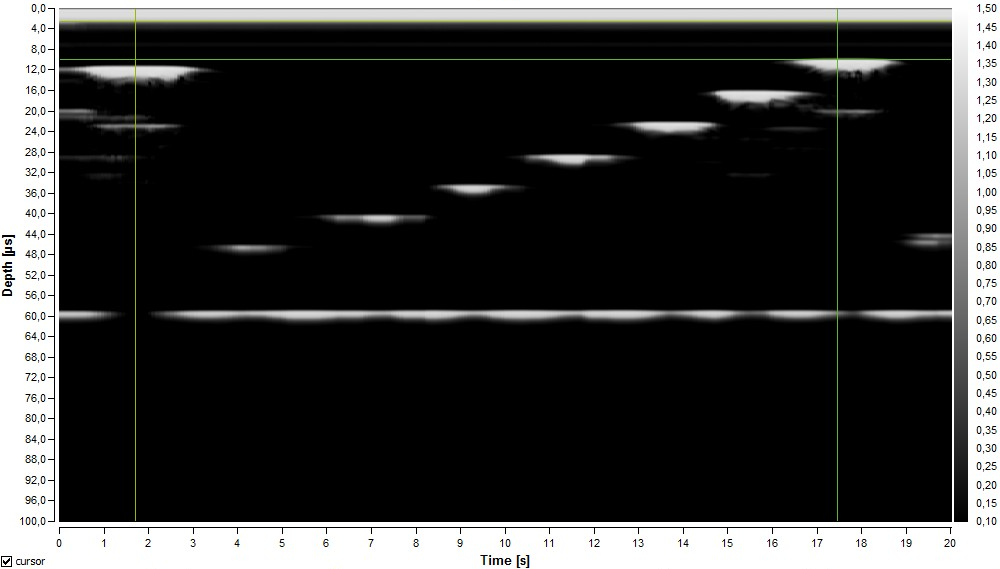
\includegraphics[width=0.7\textwidth]{images/bscanoben.png}
  \caption{Aufzeichnung des B-Scans für die Oberseite des Acrylblockes.}
  \label{fig:Boben}
\end{figure}

\begin{figure}
  \centering
  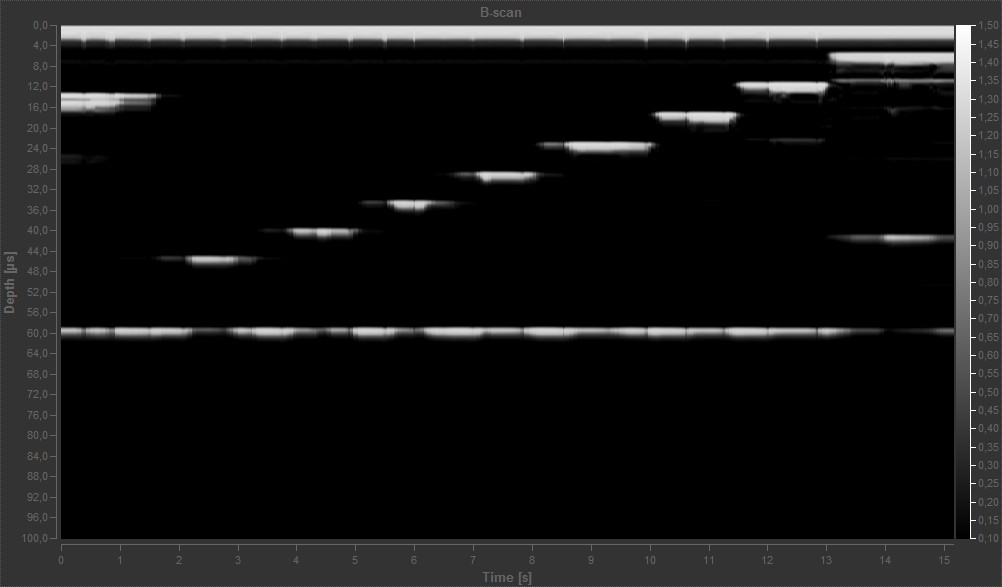
\includegraphics[width=0.7\textwidth]{images/bscanunten.png}
  \caption{Aufzeichnung des B-Scans für die Unterseite des Acrylblockes.}
  \label{fig:Bunten}
\end{figure}

\begin{table}
  \centering
  \caption{Die Messergebnisse für die Vermessung des Acrylblockes mithilfe des B-Scans.}
  \label{tab:bscan}
  \begin{tabular}[t]{c c c c c c}
   \toprule
    {Nummer} & {$t_\text{oben}$ / $\si{\micro\second}$} & {$l_\text{oben}$ / $\si{\milli\metre}$} & {$t_\text{unten}$ / $\si{\micro\second}$} & {$l_\text{unten}$ / $\si{\milli\metre}$} &  {Dicke / $\si{\milli\metre}$} \\
     \midrule
     \csvreader[no head,
     late after line=\\,
     late after last line=\\\bottomrule]%
     {data/bscantab.csv}{}%
     {$\num{\csvcoli}$ & $\num{\csvcolii}$ & $\num{\csvcoliii}$ & $\num{\csvcoliv}$ & $\num{\csvcolv}$ & $\num{\csvcolvi}$ }%
   \end{tabular}
 \end{table}

\FloatBarrier
\subsection{Untersuchung eines Herzmodells mit dem A- und TM-Scan}
Mit dem A-Scan wurden folgende Echolaufzeiten für die Schutzschicht, und die Entfernung der Membran in Ruhe und bei maximaler Auslenkung gemessen:
\begin{align*}
  t_\text{Schutzschicht} &= \SI{0.53}{\micro\second} \\
  t_\text{Ruhe} &= \SI{66.96}{\micro\second} \\
  t_\text{Maximal} &= \SI{29.11}{\micro\second} .
\end{align*}
Nun wird die Schutzschicht der Sonde von den Laufzeiten der Membran subtrahiert. Zur Bestimmung des Laufzeitunterschiedes des Mittelpunktes der Membran wird
nun $t_\text{Maximal}$ von $t_\text{Ruhe}$ abgezogen. Dann wird mittels Gleichung \eqref{eqn:wegzeit} und der aus \cite{wasser} entnommenen Schallgeschwindigkeit
für destilliertes Wasser $c=\SI{1485}{\metre\per\second}$ der maximale Höhenunterschied zu $h=\SI{28.1}{\milli\metre}$ bestimmt.
Das Schlagvolumen des Herzmodells ist nun durch das Volumen des, durch Aufpumpen der unteren Kammer entstandenen, Kugelsegments gegeben.
Das Volumen eines Kugelsegments lässt sich aus der Höhe $h$ und dem Radius $a$ des Segments mit
\begin{equation}
  V = \frac{h \pi}{6} (3a^2+h^2)
  \label{eqn:herzvol}
\end{equation}
berechnen. Mit der zuvor bestimmten Höhe und dem gemessenen Radius $a=\SI{28.825}{\milli\metre}$ wird das maximale Schlagvolumen des Herzmodells zu
\begin{equation*}
  V_\text{max}= \SI{48.30}{\milli\litre}
\end{equation*}
bestimmt.
\\
Die Messdaten und -ergebnisse zur Bestimmung des Herzzeitvolumens mit dem TM-Scan befinden sich in Tabelle \ref{tab:hzv}. Die grafische Darstellung der Messung ist in Abbildung
\ref{fig:hzv} zu sehen.
\begin{figure}
  \centering
  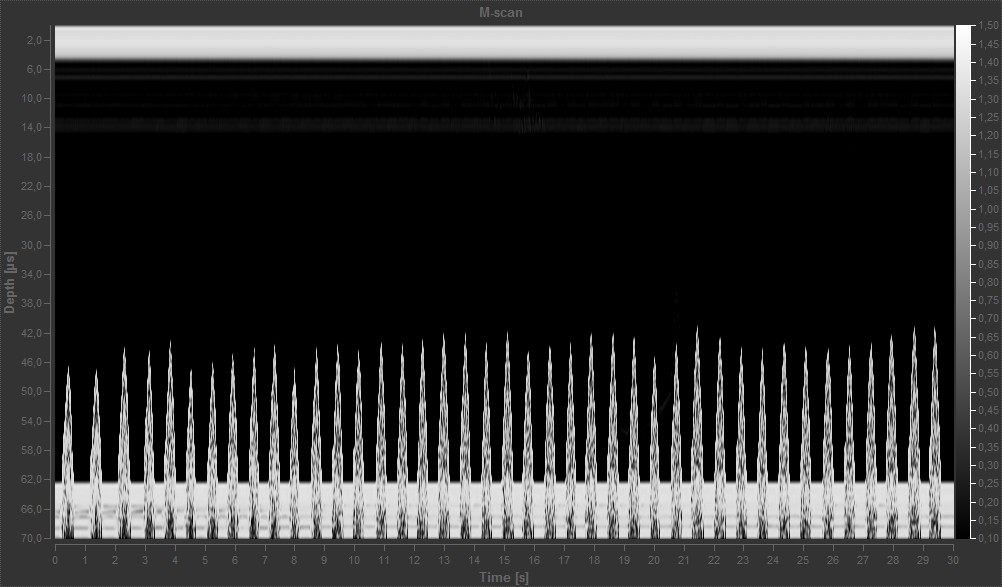
\includegraphics[scale=0.4]{images/herzreal.jpg}
  \caption{TM-Scan des Herzmodells.}
  \label{fig:hzv}
\end{figure}
Bei $t_\text{ausgelenkt}$ ist die Schutzschicht der Sonde, welche zu $\SI{4.4}{\micro\second}$ bestimmt wurde, schon abgezogen worden.
Zur Berechnung von $t_\text{Höhe}$ wurde $t_\text{ausgelenkt}$ vom Grundniveau abzüglich der Schutzschicht $t_\text{Grund}= \SI{58.12}{\micro\second}$ subtrahiert.
Aus $t_\text{Höhe}$ wird nun mittels \eqref{eqn:wegzeit} und $c=\SI{1485}{\metre\per\second}$ die Höhe $h$ berechnet.
Nun wird für jeden gemessenen Schlag das Schlagvolumen $V_\text{Schlag}$ mit \eqref{eqn:herzvol} bestimmt.
\begin{table}
  \centering
  \caption{Die Messergebnisse zur Bestimmung des Herzzeitvolumens des Herzmodells.}
  \label{tab:hzv}
  \begin{tabular}[t]{c c c c}
   \toprule
    $t_\text{ausgelenkt}$ / $\si{\micro\second}$ & $t_\text{Höhe}$ / $\si{\micro\second}$ & $h$ / $\si{\milli\metre}$ & $V_\text{Schlag}$ / $\si{\milli\litre}$ \\
     \midrule
     \csvreader[no head,
     late after line=\\,
     late after last line=\\\bottomrule]%
     {data/herztab.csv}{}%
     {$\num{\csvcoli}$ & $\num{\csvcolii}$ & $\num{\csvcoliii}$ & $\num{\csvcoliv}$}%
   \end{tabular}
 \end{table}
Die gemessenen Schlagvolumina werden nun mit
\begin{equation}
  \label{eqn:mittelwert}
  \overline{x} = \frac{1}{N} \sum_{i=1}^N x_i
\end{equation}
gemittelt und der entsprechende Fehler mit
\begin{equation}
  \label{eqn:mittelwertfehler}
  \Delta \overline{x} = \frac{1}{\sqrt{N}} \sqrt{\frac{1}{N-1} \sum_{i=1}^N (x_i - \overline{x})^2}
\end{equation}
berechnet.
So ergibt sich ein mittleres Schlagvolumen von
\begin{equation*}
  \overline{V_\text{Schlag}}= \SI{19.66\pm0.31}{\milli\litre} .
\end{equation*}
Das Herzzeitvolumen wird nun mit der aus \ref{fig:hzv} bestimmten Herzfrequenz $f_\text{Herz}=\SI{84}{\per\minute}$ durch
\begin{equation}
  HZV = \overline{V_\text{Schlag}} \cdot f_\text{Herz}
\end{equation}
zu
\begin{equation*}
  HZV=\SI{1.651\pm0.026}{\litre\per\minute}
\end{equation*}
bestimmt.
